% Part: sets-functions-relations
% Chapter: arithmetization
% Section:reals

\documentclass[../../../include/open-logic-section]{subfiles}

\begin{document}

\olfileid{sfr}{arith}{real}
\olsection{حقیقی عددی خط}

اگلا قدم ایہ وکھاؤنا اے کہ ناطق عدداں توں حقیقی عدد کِویں بنائے جان۔
ایہدے توں پہلاں ساڈے نوں سمجھنا پینا اے کہ حقیقی عدداں دی
\emph{وکھری خاصیت} کی اے۔

حقیقی عدد ناطق عدداں نال بہت رلدا ورتاؤ کردے نیں۔ (فنی طور تے دونیں
\emph{ترتیب دار میداناں} دیاں مثالاں نیں؛ ایہدی تعریف لئی
\olref[check]{orderedfield} ویکھو۔) ہُن جے تسیں
\olref[sfr][siz][]{chap} دیاں مشقاں کیتیاں نیں، تاں تہانوں پتا ہووے گا
کہ حقیقی عدد ناطق عدداں توں سختی نال ودھ نیں، یعنی
$\cardless{\Rat}{\Real}$۔ ایہ گل سب توں پہلاں کانتور نے ثابت کیتی سی۔
پر لگ بھگ ڈھائی ہزار سالاں توں ایہ معلوم اے کہ غیر ناطق عدد موجود نیں،
یعنی اوہ حقیقی عدد جیہڑے ناطق نہیں۔ واقعی:
%\footnote{نوٹ: ”$\sqrt{2}$“ صرف غیر منفی اصل جذر نوں دَسدا اے؛ دوجا حل اوہدا منفی اے۔ اگلے کجھ ورقیاں وچ اسی صرف ایسے اصل جذر اُتے غور کراں گے۔}
% PNBARI-004 ماخذ دی درستی، غیر فعال نوٹ: ریڈیکل دی علامت صرف غیر منفی اصل جذر دَسدی اے، مثبت تے منفی دونیں جذر نہیں۔
\begin{thm}\ollabel{root2irrational}
$\sqrt{2}$ ناطق نہیں، یعنی $\sqrt{2} \notin \Rat$
\end{thm}

\begin{proof}
تضاد لئی فرض کرو کہ $\sqrt{2}$ ناطق اے۔ سو
$\sqrt{2} = \nicefrac{m}{n}$، کجھ قدرتی عدد $m$ تے $n$ لئی۔ دراصل اسی
$m$ تے $n$ ایویں چُن
سکدے آں کہ کسر نوں ہور مختصر نہ کیتا جا سکے۔ ترتیب بدل کے
$m^{2} = 2n^{2}$۔ ایتھوں اسی ثبوت دو طریقیاں نال پورا کر سکدے آں:

\emph{پہلاں، ہندسی طور تے} (ٹیننبام دے پچھے چل کے)۔\footnote{ایہ
ثبوت \cite{Conway2006} وچ بیان ہویا اے۔} ایہناں مربعواں اُتے غور کرو:
\begin{center}
	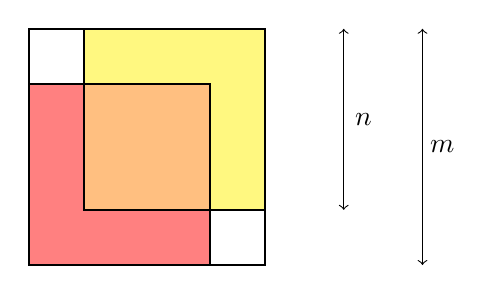
\begin{tikzpicture}
		\draw[thick] (0,0) rectangle (3,3);
		\draw[thick, fill=red!50] (0,0) rectangle (2.3,2.3);
		\draw[thick, fill=yellow!50] (0.7,0.7) rectangle (3, 3);
		\draw[thick, fill=orange!50] (0.7,0.7) rectangle (2.3, 2.3);
		\draw[<->] (4, 0.7)--(4, 3);
		\node at (4.25, 1.85) (n) {$n$};
		\draw[<->] (5, 0)--(5, 3);
		\node at (5.25, 1.5) (m) {$m$};
	\end{tikzpicture}
\end{center}
کیوں جو $m^2 = 2n^2$، ایس لئی اوہ علاقہ جتھے ضلع $n$ والے دونیں
مربع اک دوجے اُتے آندے نیں، اوس علاقے جِنّا رقبہ رکھدا اے جیہنوں دوناں
وچوں کوئی مربع نہیں ڈھکدا؛ یعنی نارنجی مربع دا رقبہ دوناں بے رنگ
مربعواں دے رقبیاں دے جوڑ دے برابر اے۔ سو جے نارنجی مربع دا ضلع $p$
تے ہر بے رنگ مربع دا ضلع $q$ ہووے، تاں $p^2 = 2q^2$۔ پر ہُن
$\sqrt{2} = \nicefrac{p}{q}$، جتھے $p < m$ تے $q < n$ تے $p, q \in
\Nat$۔ ایہ ایس گل نال ٹکراؤندا اے کہ $m$ تے $n$ نوں ممکن حد تک
چھوٹا چُنیا گیا سی۔

\emph{دوجا، رسمی طور تے۔} کیوں جو $m^{2} = 2n^{2}$، ایس توں نکلدا اے
کہ $m$ جفت اے۔ (ایہ وکھاؤنا سوکھا اے کہ جے $x$ طاق ہووے تاں $x^2$
طاق ہوندا اے۔) سو $m = 2r$، کسے $r \in \Nat$ لئی۔ ترتیب بدل کے
$2r^2 = n^2$،
		%				\begin{align*}
		%					(2r)^{2} &= 2n^{2}\\
		%					4r^{2} &= 2n^{2}\\
		%					2r^{2} &= n^{2}
		%				\end{align*}
		% PNBARI-005 ماخذ دی درستی، غیر فعال اخذ: m=2r توں بعد انگریزی تبصرے وچ غیر متعین q آ گیا سی؛ تیناں تھاواں اُتے پابند r ورتیا اے۔
سو $n$ وی جفت اے۔ ایس لئی $m$ تے $n$ دونیں جفت نیں، تے نتیجتاً
کسر $\nicefrac{m}{n}$ نوں \emph{ہور} مختصر کیتا جا سکدا اے۔
تضاد!
\end{proof}

نال دی نال، ایہ شکلی ثبوت سانوں \olref[his][set][mythology]{sec} دے
مواد ول واپس جان دی سہولت دیندا اے۔ ٹیننبام (1927--2006) پورے طور تے
جدید ریاضی دان سی؛ پر ایہ ثبوت بے شک سوہنا، پوری طرح کڑا، تے ہندسی
وجدان نوں ورتن والا اے!

بہرحال، حقیقی عدد ناطق عدداں توں ”ہور وسیع“ نیں۔ اک معنٰی وچ ناطق
عددی خط وچ ”خلا“ نیں، تے حقیقی عدد اوہناں نوں بھر دے نیں۔ وائرسٹراس
نے سمجھیا کہ ایہ حقیقی عدداں دی اکّو خاصیت بیان کردا اے، جیہڑی اوہناں
نوں ناطق عدداں توں وکھرا کردی اے، یعنی تکمیلیت دی خاصیت:
\emph{حقیقی عدداں دے ہر غیر خالی سیٹ، جیہدی کوئی بالائی حد ہووے، دی اک
سب توں چھوٹی بالائی حد ہوندی اے۔}

ایہ ویکھنا سوکھا اے کہ ناطق عدداں کول تکمیلیت دی خاصیت نہیں۔ مثال لئی
$\sqrt{2}$ توں چھوٹے ناطق عدداں دے ایس سیٹ اُتے غور کرو، یعنی:
\[
	\Setabs{p \in \Rat}{p^2 < 2 \text{ یا }p < 0}
\]
ایس دی ناطق عدداں وچ اک بالائی حد اے؛ مثال لئی ایہدے !!{element}s
سارے $3$ توں چھوٹے نیں۔
% PNBARI-003 ماخذ دی درستی: element ٹوکن دے فوراً بعد اک بے محل < سی؛ کوئی کھبا operand نہیں، تے جملہ آپ دَسدا اے کہ سارے رکن 3 توں چھوٹے نیں۔
پر ایہدی سب توں چھوٹی بالائی حد کی اے؟ اسی
”$\sqrt{2}$“ آکھنا چاہنے آں؛ پر ہُنّے ویکھیا اے کہ $\sqrt{2}$
\emph{ناطق نہیں}۔ تے $\sqrt{2}$ توں وڈا کوئی \emph{سب توں چھوٹا}
ناطق عدد نہیں۔ سو ایس سیٹ دی بالائی حد تاں اے، پر سب توں چھوٹی بالائی
حد نہیں۔ لہٰذا ناطق عدداں کول تکمیلیت دی خاصیت نہیں۔

ایہدے برعکس، استمراری خط کول ”اصولی طور تے“ تکمیلیت دی خاصیت ہونی
چاہیدی اے۔ اسی صرف ایہ نہیں چاہندے کہ $\sqrt{2}$ حقیقی عدد ہووے؛ اسی
ناطق عددی خط دے سارے ”خلا“ بھرنے چاہنے آں۔ بلکہ اسی چاہنے آں کہ
استمراری خط دے اپنے اندر کوئی ”خلا“ نہ ہووے۔ تکمیلیت توں سانوں عین
ایہو ملے گا۔

\end{document}
